\documentclass[12pt,a4paper]{article}

\usepackage[utf8]{inputenc}
\usepackage[T2A]{fontenc}
\usepackage[ukrainian]{babel}
\usepackage{geometry}
\geometry{
    left=2cm,
    right=2cm,
    top=2cm,
    bottom=2cm
}

\usepackage[table]{xcolor}
\usepackage{amsmath}
\usepackage{graphicx}
\usepackage{subcaption}
\usepackage{multirow}
\usepackage{makecell}
\usepackage{pdflscape}
\usepackage{array}
\newcolumntype{C}[1]{>{\centering\arraybackslash}m{#1}}

\usepackage[
  unicode,
  pdftitle={ІО-41, Давидчук А.М., Організація баз даних, Лабораторна робота №1},
  pdfauthor={Давидчук Артем},
  pdfsubject={Організація баз даних}
]{hyperref}

\begin{document}

    \begin{titlepage}

    \begin{center}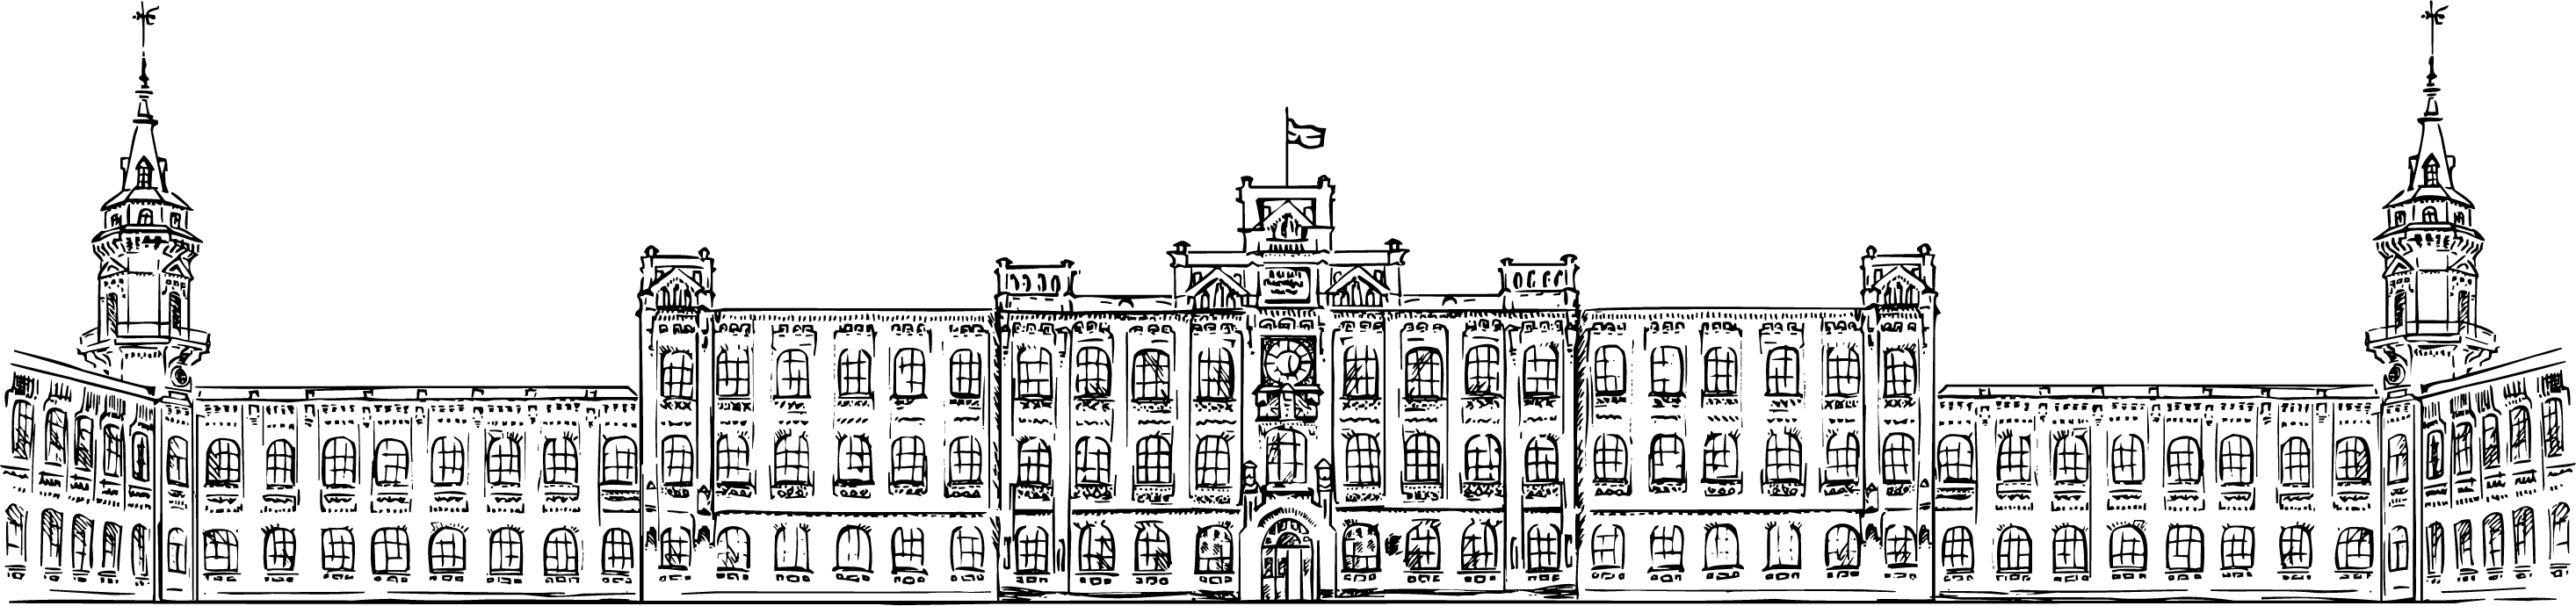
\includegraphics[width=0.7\textwidth]{../../../TITLES/letterhead.png}\end{center}

    \begin{center}
        \large Національний технічний університет України\\
        «Київський політехнічний інститут імені Ігоря Сікорського»\\[1em]
        Факультет інформатики та обчислювальної техніки\\
        Кафедра обчислювальної техніки
    \end{center}

    \vfill

    \begin{center}
        \textbf{\LARGE Організація баз даних}\\[2em]
        \textbf{\Large Лабораторна робота №1}\\[0.5em]
        «Збір вимог та розробка схем ER» 
    \end{center}

    \vfill

    \begin{flushright}
        Виконав: студент 1 курсу ФІОТ, гр. ІО-41\\
        \textit{Давидчук А. М.}\\
        Залікова книжка № 4106\\[1em]
        Перевірив: \textit{Русінов В.\,В.}
    \end{flushright}

    \vfill

    \begin{center}Київ --- 2026\end{center}

    \end{titlepage}

    \noindent
    \textbf{\underline{Тема:}} «Збір вимог та розробка схем ER».

    \vspace{1em}

    \noindent
    \textbf{\underline{Мета:}} Навчитися збирати та документувати вимоги до інформаційної системи, виділяти з них ключові сутності, їх атрибути та зв’язки, а також побудувати концептуальну ER-діаграму (Entity–Relationship Diagram), що відображає модель даних і слугує основою для подальшого проєктування та реалізації бази даних у СУБД.

    \begin{center} \textbf{\large Хід роботи} \end{center}

    \noindent
    Змоделюємо систему чата клієнта із певною моделлю ШІ -- система повинна:

    \begin{enumerate}
        \item зберігати історію чатів і повідомлень;
        \item дозволяти прикріплювати файли до повідомлень;
        \item фіксувати, якою моделлю і з якими параметрами була згенерована відповідь.
    \end{enumerate}

    \noindent
    Звідси зацікавлені сторони:

    \begin{enumerate}
        \item Користувач (User): створює чати, надсилає повідомлення, прикріплює файли;
        \item AI модель: генерує відповіді, зберігає метадані генерації (модель, параметри).
    \end{enumerate}

    \noindent
    Визначимо також основні сценарії, які можуть відбуватись у нашій системі:

    \begin{enumerate}
        \item Користувач створює новий чат;
        \item Користувач надсилає повідомлення в чат;
        \item Користувач прикріплює файл до повідомлення (картинка/пдф/код тощо);
        \item Система генерує відповідь AI і зберігає її разом з метаданими генерації.
    \end{enumerate}

    \noindent
    Тепер визначимо основні сутності, які є частиною цієї системи (відповідно до ER-моделі):

    \vspace{1em}

    \noindent
    \textbf{User} (користувач):

    \begin{enumerate}
        \item \texttt{user\_id} (PK) -- унікальний ідентифікатор користувача;
        \item \texttt{firstName} -- ім'я;
        \item \texttt{secondName} -- прізвище;
        \item \texttt{userName} -- нікнейм користувача;
        \item \texttt{email} -- електронна пошта;
        \item \texttt{country} -- країна;
        \item \texttt{created\_at} -- дата створення облікового запису.
    \end{enumerate}

    \vspace{0.75em}

    \noindent
    \textbf{Chat} (чат):

    \begin{enumerate}
        \item \texttt{chat\_id} (PK) -- унікальний ідентифікатор чату;
        \item \texttt{ownerUser\_id} (FK $\rightarrow$ \texttt{User.user\_id}) -- власник чату;
        \item \texttt{title} -- назва чату;
        \item \texttt{created\_at} -- дата створення чату.
    \end{enumerate}

    \vspace{0.75em}

    \noindent
    \textbf{Message} (повідомлення у чаті):

    \begin{enumerate}
        \item \texttt{message\_id} (PK) -- унікальний ідентифікатор повідомлення;
        \item \texttt{chat\_id} (FK $\rightarrow$ \texttt{Chat.chat\_id}) -- чат, до якого належить повідомлення;
        \item \texttt{role} -- тип повідомлення (\texttt{user} або \texttt{AImodel});
        \item \texttt{content} -- текст повідомлення;
        \item \texttt{created\_at} -- дата/час створення повідомлення.
    \end{enumerate}

    \vspace{0.75em}

    \noindent
    \textbf{Attachment} (вкладення до повідомлення):

    \begin{enumerate}
        \item \texttt{attachment\_id} (PK) -- унікальний ідентифікатор вкладення;
        \item \texttt{message\_id} (FK $\rightarrow$ \texttt{Message.message\_id}) -- повідомлення, до якого прикріплено файл;
        \item \texttt{file\_name} -- назва файлу;
        \item \texttt{size\_bytes} -- розмір файлу (у байтах);
        \item \texttt{path} -- шлях/посилання на файл у сховищі;
        \item \texttt{uploaded\_at} -- дата/час завантаження.
    \end{enumerate}

    \vspace{0.75em}

    \noindent
    \textbf{AImodel} (модель ШІ):

    \begin{enumerate}
        \item \texttt{model\_id} (PK) -- унікальний ідентифікатор моделі;
        \item \texttt{modelName} -- назва моделі;
        \item \texttt{modelVersion} -- версія моделі.
    \end{enumerate}

    \vspace{0.75em}

    \noindent
    \textbf{Generation} (метадані генерації відповіді ШІ):

    \begin{enumerate}
        \item \texttt{generaion\_id} (PK) -- унікальний ідентифікатор події генерації;
        \item \texttt{model\_id} (FK $\rightarrow$ \texttt{AImodel.model\_id}) -- модель, яка згенерувала відповідь;
        \item \texttt{message\_id} (FK $\rightarrow$ \texttt{Message.message\_id}) -- повідомлення-відповідь (\texttt{role=AImodel}), для якого збережено метадані;
        \item \texttt{parameters} -- параметри генерації у форматі \texttt{JSONB} (PostgreSQL), що містять ключ--значення (наприклад, \texttt{temperature}, \texttt{top\_p}, \texttt{max\_tokens} тощо);
        \item \texttt{created\_at} -- дата/час створення запису про генерацію.
    \end{enumerate}

    \newpage

    \noindent
    \textbf{Пояснення зв'язків між сутностями.}

    \begin{enumerate}
        \item \texttt{User (1) -- (M) Chat:} один користувач може створювати довільну кількість чатів (включно з нулем), а кожен чат має рівно одного власника.
        \item \texttt{Chat (1) -- (M) Message:} один чат містить довільну кількість повідомлень (включно з нулем), а кожне повідомлення належить рівно одному чату.
        \item \texttt{Message (1) -- (0..M) Attachment:} одне повідомлення може не мати вкладень або мати багато вкладень; при цьому кожне вкладення прикріплене рівно до одного повідомлення.
        \item \texttt{Message (1) -- (0..1) Generation:} для повідомлення типу \texttt{AImodel} може існувати один запис метаданих генерації (модель та параметри), а для повідомлення типу \texttt{user} запис \texttt{Generation} відсутній.
        \item \texttt{AImodel (1) -- (0..M) Generation:} одна й та сама модель може використовуватись у багатьох генераціях, але кожна конкретна генерація виконується рівно однією моделлю.
    \end{enumerate}

    \vspace{0.75em}

    \noindent
    \textbf{ER-діаграма системи:}

    \begin{figure}[h!]
        \centering
        \includegraphics[width=0.8\textwidth]{media/ERD.pdf}
        \caption{ER-діаграма системи чата з моделлю ШІ}
    \end{figure}

    \vspace{0.75em}

    \noindent
    \textbf{Припущення та обмеження.}
    \begin{itemize}
        \item Групові чати не підтримуються: у кожному чаті може писати лише його власник (\texttt{Chat.ownerUser\_id}). Отже, авторство всіх повідомлень з \texttt{role=user} визначається через власника чату.
        \item Метадані генерації зберігаються лише для повідомлень з \texttt{role=AImodel}: для таких повідомлень існує запис у \texttt{Generation}, для \texttt{role=user} запис \texttt{Generation} відсутній.
        \item Вкладення існує лише як прикріплене до повідомлення: кожен запис \texttt{Attachment} пов'язаний з рівно одним \texttt{Message} і не може існувати ``самостійно'' поза повідомленням.
        \item Параметри генерації \texttt{parameters} реалізуються в PostgreSQL типом \texttt{JSONB} як розширюваний набір пар ``ключ--значення'' (наприклад, \texttt{temperature}, \texttt{top\_p}, \texttt{max\_tokens}, \texttt{seed}, \texttt{stop} тощо).
    \end{itemize}

    \begin{center} \textbf{\large Висновок} \end{center}

    У ході лабораторної роботи було зібрано та сформульовано вимоги до інформаційної системи чата з моделлю ШІ, визначено ключові сутності, їх атрибути та бізнес-правила. На основі цього побудовано концептуальну ER-діаграму, що відображає структуру зберігання чатів, повідомлень, вкладень і метаданих генерації відповідей. Отримана модель може бути використана як основа для подальшого проєктування та реалізації бази даних у PostgreSQL.

\end{document}